%! Author = Ryan Coslove (rmc326), Shane Ngai (sn718), and Bryan Sun (bs893)
%! Due Date = 11/12/2021

\documentclass{article}

\setlength{\headsep}{0.75 in}
\setlength{\parindent}{0 in}
\setlength{\parskip}{0.1 in}

%=====================================================
% Add PACKAGES Here (You typically would not need to):
%=====================================================

\usepackage{xcolor}
\usepackage[margin=1in]{geometry}
\usepackage{amsmath,amsthm,amssymb}
\usepackage{fancyhdr}
\usepackage{enumitem}
\usepackage{algorithm}
\usepackage{algpseudocode}
\usepackage{graphicx}
\usepackage{xspace}
\usepackage{subcaption}

%=====================================================
% Ignore This Part (But Do NOT Delete It:)
%=====================================================

\theoremstyle{definition}
\newtheorem{problem}{Problem}
\def\fline{\rule{0.75\linewidth}{0.5pt}}
\newcommand{\finishline}{\begin{center}\fline\end{center}}
\newtheorem*{solution*}{Solution}
\newenvironment{solution}{\begin{solution*}}{{\finishline} \end{solution*}}
\newcommand{\thisdate}{November 12, 2021}
\newcommand{\thissemester}{\textbf{Rutgers: Fall 2021}}
\newcommand{\thiscourse}{CS 440: Intro to AI} 
\newcommand{\thishomework}{Number} 
\newcommand{\thisname}{Name} 

\headheight 40pt              
\headsep 10pt
\pagestyle{fancy}

\newcommand{\thisheading}{
   \noindent
   \begin{center}
   \framebox{
      \vbox{\vspace{2mm}
    \hbox to 6.28in { \textbf{\thiscourse \hfill \thissemester} }
       \vspace{4mm}
       \hbox to 6.28in { {\Large \hfill Homework \#\thishomework \hfill} }
       \vspace{2mm}
         \hbox to 6.28in { { \hfill \thisdate  \hfill} }
       \vspace{2mm}
       \hbox to 6.28in {{Names: \thisname \hfill}}
      \vspace{2mm}}
      }
   \end{center}
   \bigskip
}

%=====================================================
% Some useful MACROS (you can define your own in the same exact way also)
%=====================================================


\newcommand{\ceil}[1]{{\left\lceil{#1}\right\rceil}}
\newcommand{\floor}[1]{{\left\lfloor{#1}\right\rfloor}}
\newcommand{\prob}[1]{\Pr\paren{#1}}
\newcommand{\expect}[1]{\Exp\bracket{#1}}
\newcommand{\var}[1]{\textnormal{Var}\bracket{#1}}
\newcommand{\set}[1]{\ensuremath{\left\{ #1 \right\}}}
\newcommand{\poly}{\mbox{\rm poly}}


%=====================================================
% Fill Out This Part With Your Own Information:
%=====================================================
\renewcommand{\thishomework}{2} %Homework number
\renewcommand{\thisname}{Ryan Coslove (rmc326), Shane Ngai (sn718),  Bryan Sun (bs893)} % Enter your name here



\begin{document}

\thisheading
\vspace{-0.75cm}


\begin{problem} %problem 1
	Trace the operation of A* search (the tree version) applied to the problem of getting to Bucharest from Lugoj using the straight-line distance heuristic. That is, show the sequence of nodes that the algorithm will consider and the $f , g,$ and $h$ score for each node. You don’t need to draw the graph, just right down a sequence  $(city, f (city), g(city), h(city))$ in the order in which the nodes are expanded.

\end{problem}

\begin{solution}
	\item  

	\begin{figure}[h!]
			\centering
			\IfFileExists{HW2 Prob 1 Table.png}{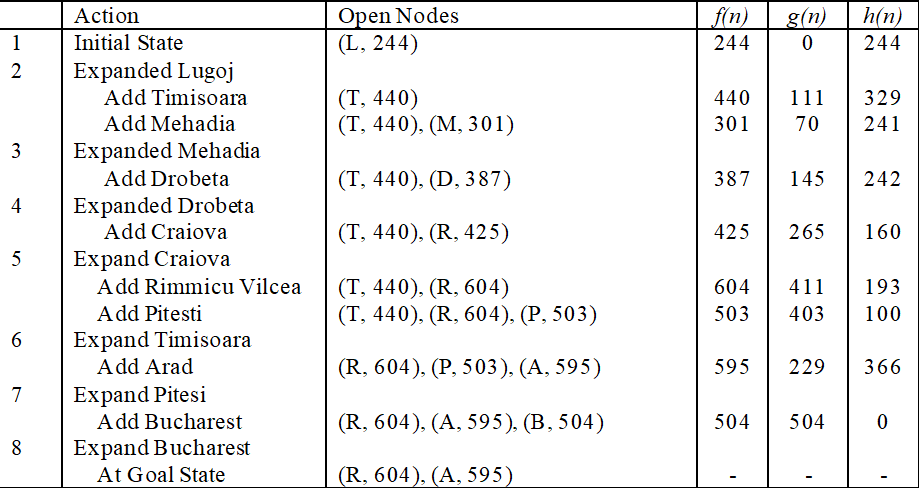
\includegraphics[width=0.9\textwidth]{HW2 Prob 1 Table.png}}
		 
		\end{figure}
	
\end{solution}

\begin{problem} %problem 2
	Consider a state space where the start state is number 1 and each state k has two successors:
numbers 2k and 2k + 1.
\item (a) Suppose the goal state is 11. List the order in which states will be visited for breadthfirst search, depth-limited search
with limit 3, and iterative deepening search.
\item (b) How well would bidirectional search work on this problem? List the order in which states will be visited. What is the
branching factor in each direction of the bidirectional search?

\end{problem}

\begin{solution}
	\item a.) (tree diagram below)
		\begin{figure}[h!]
			\centering
			\IfFileExists{HW2 Prob 2 Tree.png}{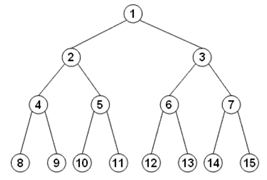
\includegraphics[width=0.4\textwidth]{HW2 Prob 2 Tree.png}}
		 
		\end{figure}
	\item  BFS: $1 \rightarrow 2 \rightarrow 3 \rightarrow 4 \rightarrow 5 \rightarrow 6 \rightarrow 7 \rightarrow 8 \rightarrow 9 \rightarrow 10 \rightarrow 11$
	\item DFS: $1 \rightarrow 2 \rightarrow 4 \rightarrow 8 \rightarrow 9 \rightarrow 5 \rightarrow 10 \rightarrow 11$
	\item IDS: $1; 1 \rightarrow 2 \rightarrow 3; 1\rightarrow 2 \rightarrow 4 \rightarrow 5 \rightarrow 3 \rightarrow 6 \rightarrow 7; 1 \rightarrow 2 \rightarrow 4 \rightarrow 8 \rightarrow 9 \rightarrow 5 \rightarrow 10 \rightarrow 11.$

	\item b.) Birectional search would work well for this problem. The predecessor of each state $x$ is $\frac{x}{2}$, which is very easy to compute. If we use BFS in both forward and backward directions, the search steps are shown in the table below. Notice that the algorithm stops when the search in the backward direction visits node 5 since 5 is in the fringe of the forward direction. 
	\item 
		\begin{figure}[h!]
			\centering
			\IfFileExists{HW2 Prob 2 Table.png}{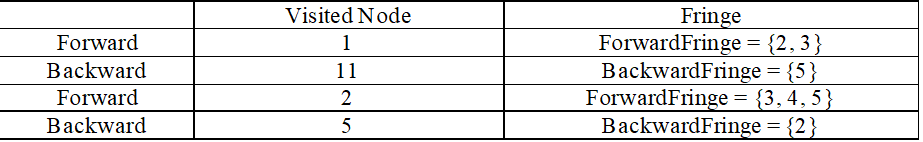
\includegraphics[width=0.9\textwidth]{HW2 Prob 2 Table.png}}
		 
		\end{figure}
	\item The branching factors are as follows: 2 in the forward direction. 1 in the backward direction. 
	
\end{solution}

\begin{problem} %problem 3
	Which of the following statements are correct and which ones are wrong?
	\item a.) Breadth-first search is a special case of uniform-cost search.
	\item b.) Depth-first search is a special case of best-first tree search.
	\item c.) Uniform-cost search is a special case of A* search.
	\item d.) Depth-first graph search is guaranteed to return an optimal solution.
	\item e.) Breadth-first graph search is guaranteed to return an optimal solution.
	\item f.) Uniform-cost graph search is guaranteed to return an optimal solution.
	\item g.) A* graph search is guaranteed to return an optimal solution if the heuristic is consistent.
	\item h.) A* graph search is guaranteed to expand no more nodes than depth-first graph search if the heuristic is consistent.
	\item i.) A* graph search is guaranteed to expand no more nodes than uniform-cost graph search if the heuristic is consistent.

\end{problem}

\begin{solution}
	\item a.) Correct
	\item b.) Correct
	\item c.) Correct
	\item d.) Incorrect
	\item e.) Incorrect
	\item f.) Correct
	\item g.) Correct
	\item h.) Incorrect
	\item i.) Correct 

\end{solution}


\begin{problem} %problem 4
	Iterative deepening is sometimes used as an alternative to breadth first search. Give one advantage of iterative deepening over BFS, and give one disadvantage of iterative deepening as compared with BFS. Be concise and specific.

\end{problem}

\begin{solution}
	\item The advantage of iterative deepending over BFS is iterative requires less memory.
	\item The disadvantage of iterative deepening over BFS is iterative repeats computations so it requires additional run time. 

\end{solution}

\begin{problem} %problem 5
	Prove that if a heuristic is consistent, it must be admissible. Construct an example of an admissible heuristic that is not consistent. (Hint: you can draw a small graph of 3 nodes and write arbitrary cost and heuristic values so that the heuristic is admissible but not consistent).

\end{problem}

\begin{solution}
	\item For every node $n$ and every success or $n?$ of a heuristic A* if and only if consistent of $n$ any location by generated of action of $a$. 
   	\item \begin{center}
       		 $h(n)? c(n, a, n?) + h(n?)$ 
  		 \end{center}
	\item  Proof by induction that of one of the number of nodes of $k$, the shortest path of $n$ to the goal state from $k=1$.
	\item Let $n?$ be the node of the goal. $h(n)$ then ? $c(n, a, n)$. The inductive case for:
	\item Assume $n?$ is on the shortest path of $k-path$ steps from the goal $h(n?)$ is admissible by:
	\item \begin{center}
       		 $h(n)? c(n, a, n?) + h(n?)?c(n, a, n) + h^*(n?) =  h^*(n)$
		\end{center}
	\item Therefore $k+1$ at $h(n)$ from steps that are admissible of goal. The text proves that when a heuristic is consistent, then the function or cost of any path is non-decreasing and admissible. 
	\item An example of a heuristic that is admissible and not consistent is in the graph below. We start at point $s$ and the goal is $h(s) = 10$; $f(s) = 10$; $h(a) = 7$; $f(a) = 1+7=8$; $h(b) = 5$; $f(b) = 1+5 = 6$; $f(t) = 11$
		\begin{figure}[h!]
			\centering
			\IfFileExists{HW2 Prob 5.png}{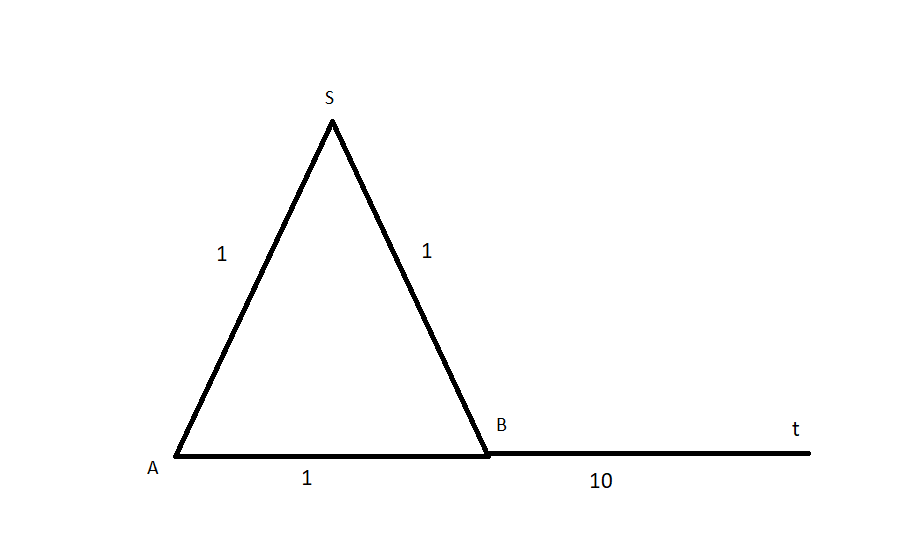
\includegraphics[width=0.7\textwidth]{HW2 Prob 5.png}}
		 
		\end{figure}

\end{solution}

\begin{problem} %problem 6
	\item In a CSP search, explain why it is a good heuristic to choose the variable that is most constrained but the value that is least constraining. 

\end{problem}

\begin{solution}
	\item It is a good heuristic to choose the variable that is most constrained because such variables are likely to cause a failure and it is more efficient to fail as early as possible. The least constraining value heuristic is good because there will be a possibility that more number of future assignments will take place that avoid conflict.  

\end{solution}

\begin{problem} %problem 7
	\item Consider the following game tree, where the first move is made by the MAX player and the second move is made by the MIN player.
		\item a.) What is the best move for the MAX player using the minimax procedure?
		\item b.) Perform a left-to-right (left branch first, then right branch) alpha-beta pruning on the tree. That is, draw only the parts of the tree that are visited and don't draw branches that are cut off (no need to show the alpha or beta moves)
		\item c.) Do the same thing as the previous question, but with a right-to-left ordering of the actions. Discuss why different pruning occurs.

\end{problem}

\begin{newpage}
\end{newpage}

\begin{solution}
	\item a.)
	\item \begin{figure}[h!]
			\centering
			\IfFileExists{HW2 Prob 7a.png}{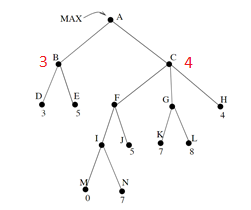
\includegraphics[width=0.5\textwidth]{HW2 Prob 7a.png}}
		 	\item 
			\caption{Figure for 7a.}
		\end{figure}
	\item The best move for MAX player is A to C (as H=4 and B to D=3)

	\item b.)
	\item \begin{figure}[h!]
			\centering
			\IfFileExists{HW2 Prob 7 b.jpg}{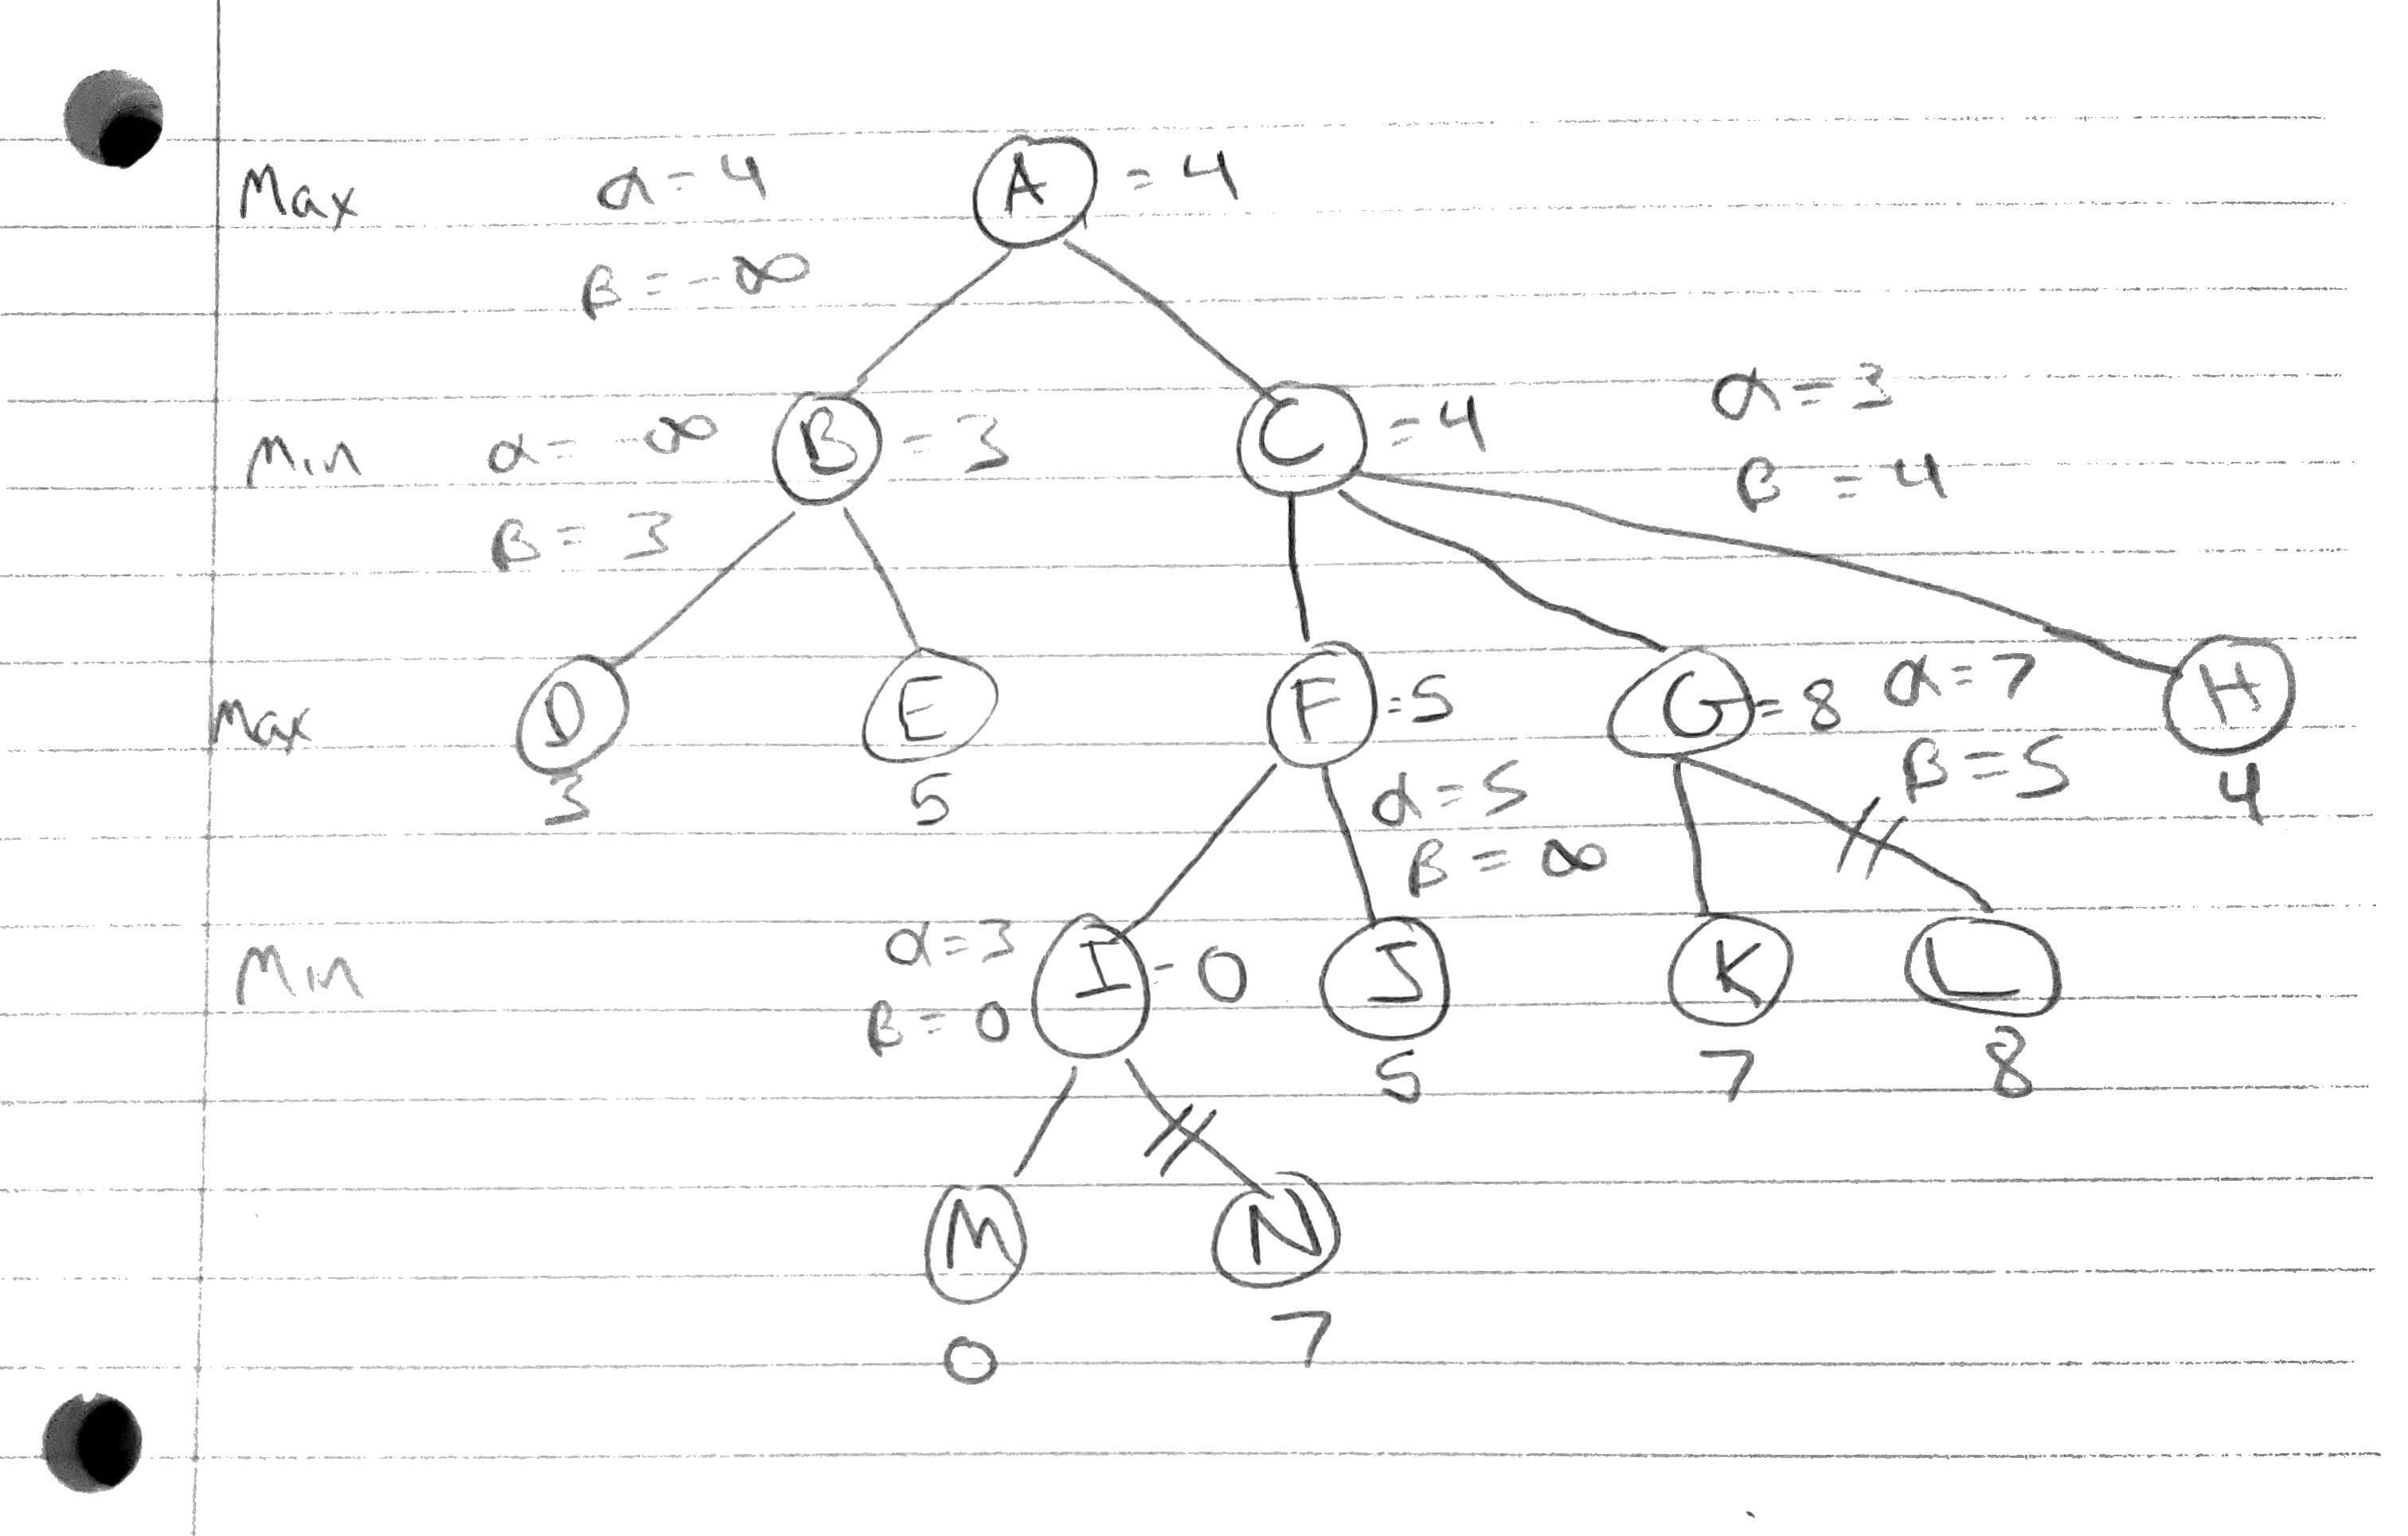
\includegraphics[width=0.7\textwidth]{HW2 Prob 7 b.jpg}}
			\item 
		 	\caption{Figure for 7b.}
		\end{figure}
	
	\item  c.)
	\item \begin{figure}[h!]
			\centering
			\IfFileExists{HW2 Prob 7 c.jpg}{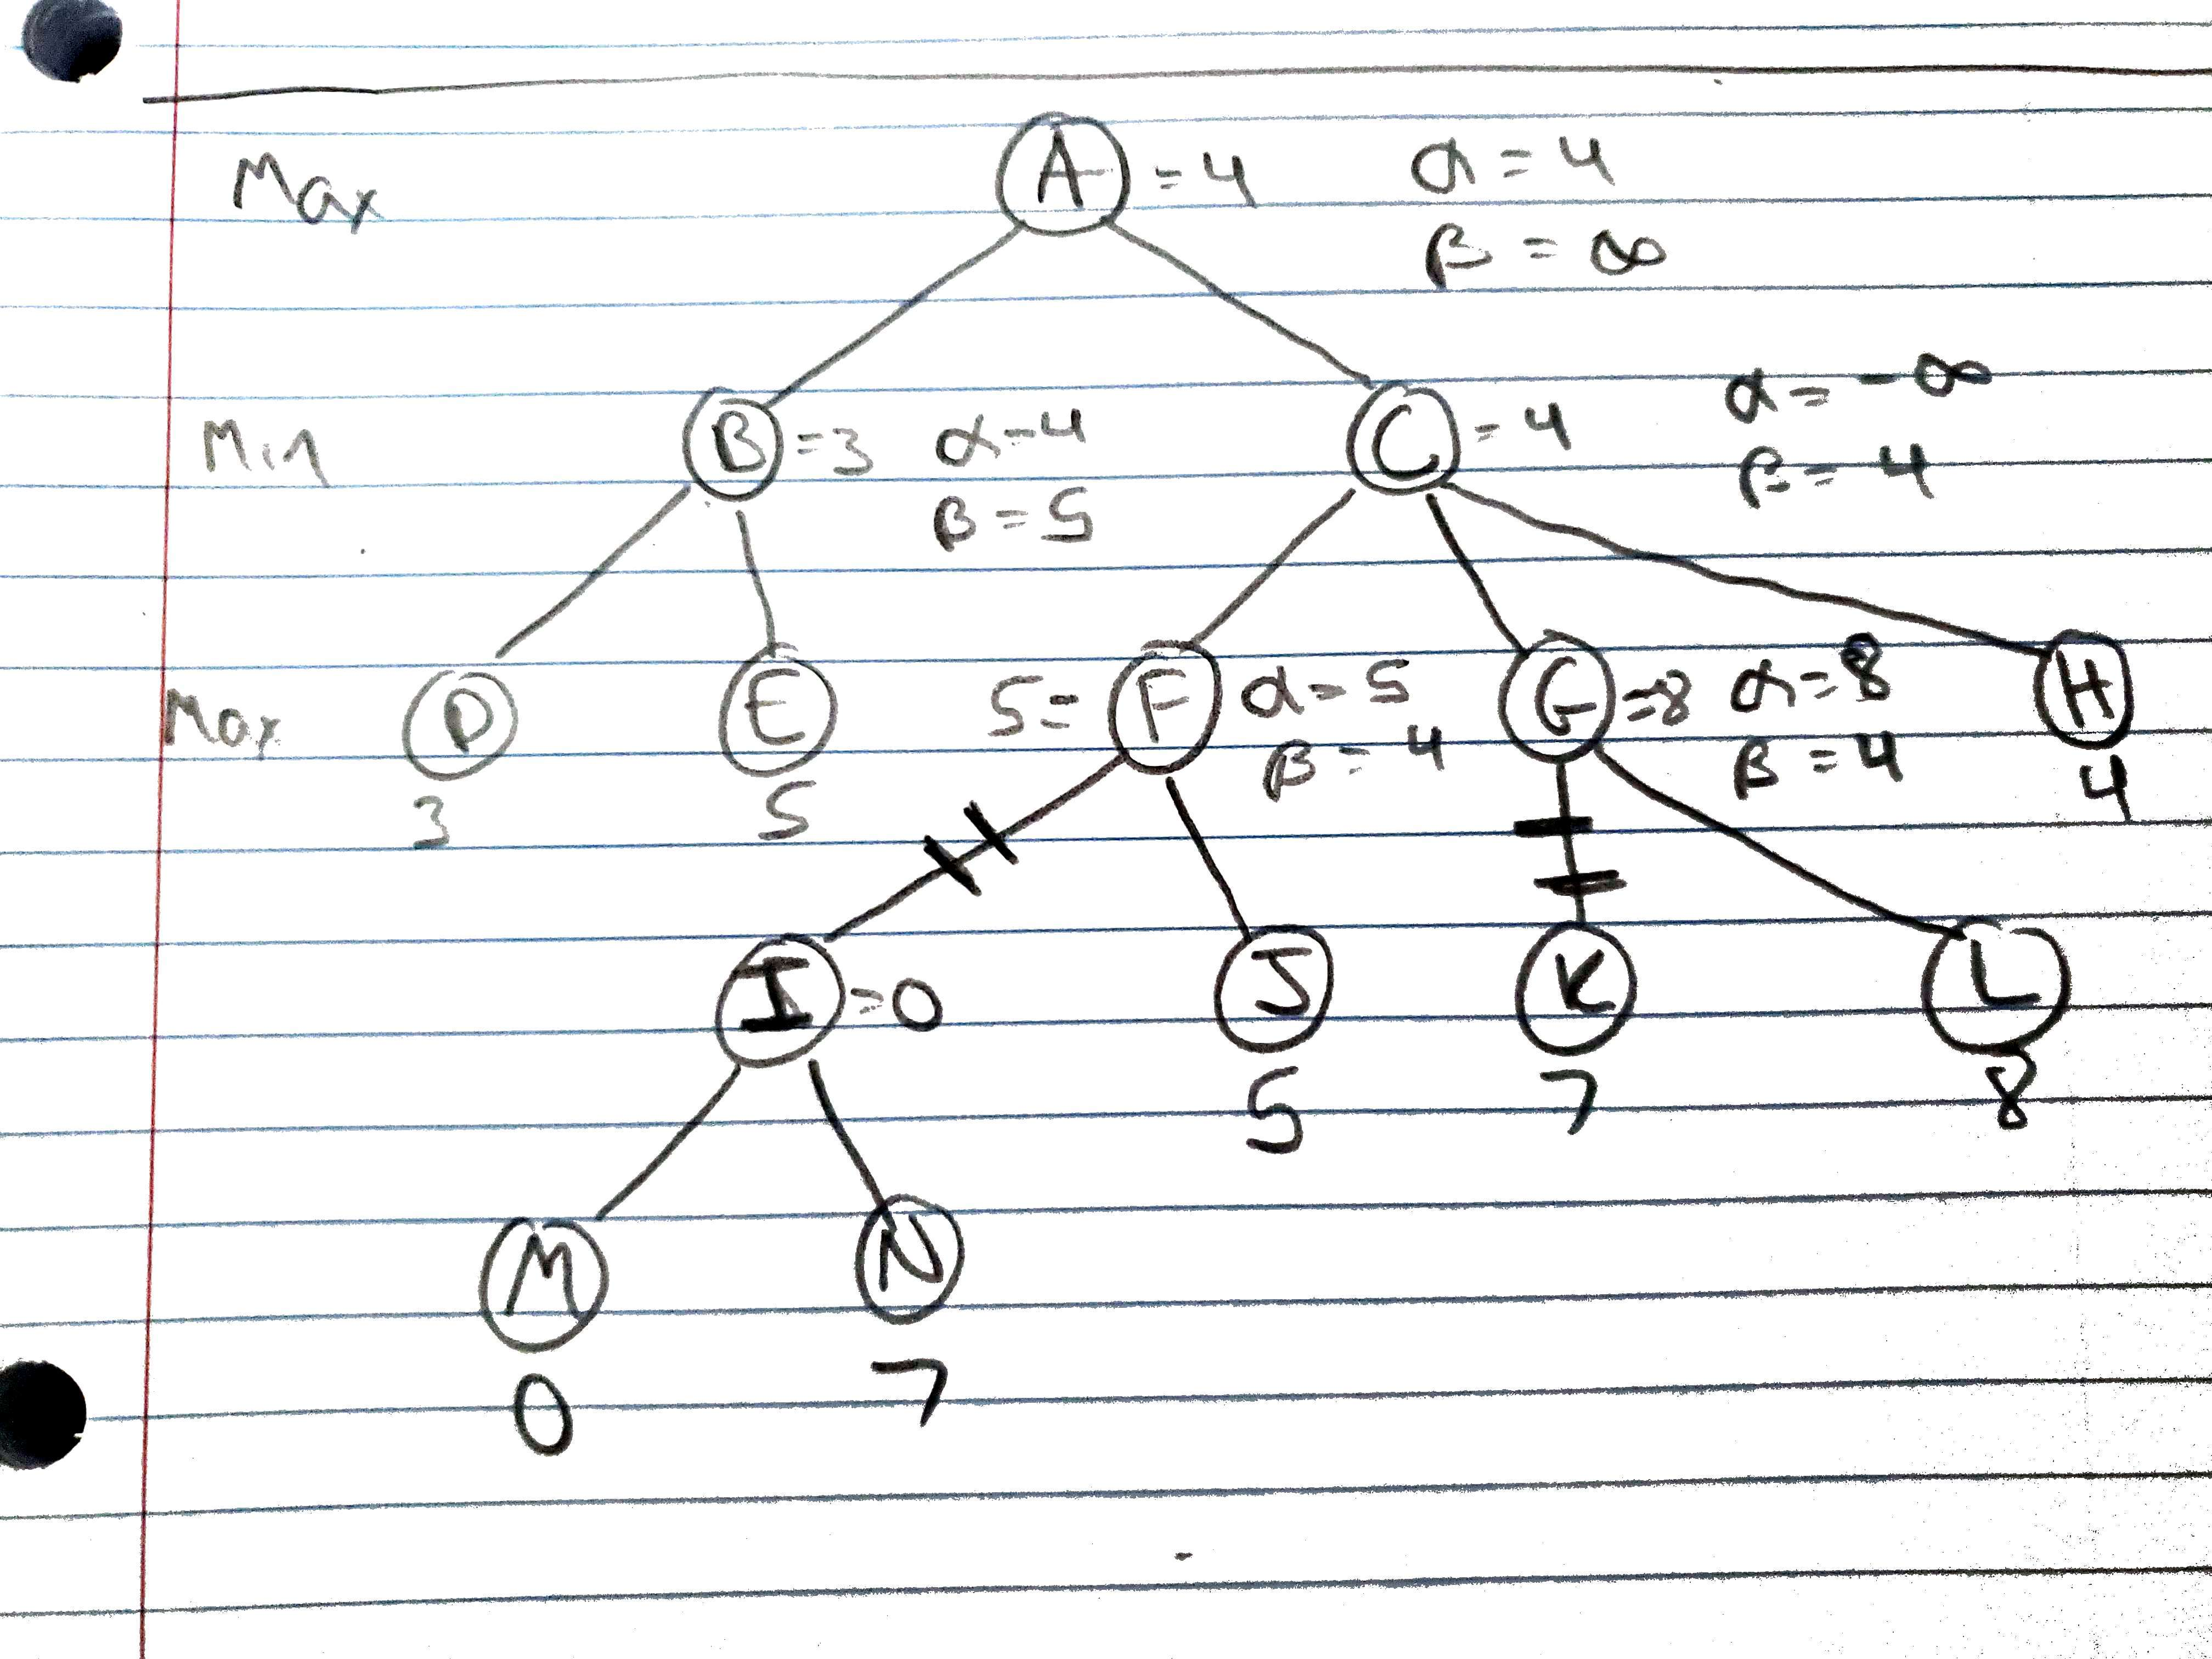
\includegraphics[width=0.7\textwidth]{HW2 Prob 7 c.jpg}}
			\item 
		 	\caption{Figure for 7c.}
		\end{figure}
	\item Alpha-Beta pruning from right to left traversing is different from left to right because the condition of alpha beta pruning states that if a node has alpha $>=$ beta, then the other branch of that node will not traverse. This would be the left branch in case of right to left, right branch in case of left to right. That path instead will be pruned. So while this condition is true, the right or left path will be cut resulting in different pruning during traversal. 

\end{solution}

\begin{problem} %problem 8
    Which of the following are admissible, given admissible heuristics $h_1$,$h_2$? Which of the following are consistent, given consistent heuristics $h_1$,$h_2$ Justify your answer. 
    \item a) $h(n) = min\{h_1(n),h_2(n)\}$
    \item b) $h(n) = wh_1(n)+(1-w)h_2(n)$, where $0 \le w \le 1$
    \item c) $h(n) = max\{h_1(n),h_2(n)\}$

\end{problem}

\begin{solution}
	\item a.) Given, $h(n) = min\{h_1(n),h_2(n)\}$. This is admissible because $h_1(n) \leq h^*(n)$. It is always true that $min(h_1(n), \infty) \leq h^*(n)$. This is also consistent because the cost will always be lower than the max cost of the path. 
	\item b.) $h_4(n) = wh_1(n) + (1-w)h_2(n)$, where $0 \leq w \leq 1$. Since $h_1$ and $h_2$ are admissible, $h_4$ is also admissible for $0 \leq w \leq 0.5$.This is also consistent because the cost from  $0 \leq w \leq 0.5$ will be less than the cost where $0 \leq w \leq 1$.
	\item c.) $h_5(n) = max\{h_1(n), h_2(n)\}$. This is admissible because if $h_1(n) \leq h^*(n)$ and $h_2(n) \leq h^*(n)$, we can deduce $ max\{h_1(n), h_2(n)\} \leq h^*(n)$. This is not consistent because the cost of the path may be higher than the optimal path. 
    
    
\end{solution}

\begin{problem} %problem 9
    Stimulated annealing is an extension of hill climbing, which uses randomness to avoid getting stuck in local maxima and plateaux.
    
    \item a) For what types of problems will hill climbing work better than simulated annealing? In other words, when is the random part of simulated annealing not necessary?
    \item b) For what types of problems will randomly guessing the state work just as well as simulated annealing? In other words, when is the hill-climbing part of simulated annealing not necessary?
    \item c) Reasoning from your answers to parts (a) and (b) above, for what types of problems is simulated annealing a useful technique? In other terms, what assumptions about the shape of the value function are implicit in the design of simulated annealing?
    \item d) As defined in your textbook, simulated annealing returns the current state when the end of the annealing schedule is reached and if the annealing schedule is slow enough. Given that we know the value (measure of goodness) of each state we visit, is there anything smarter we could do?
    \item e) Simulated annealing requires a very small amount of memory, just enough to store two states: the current state and the proposed next state. Suppose we had enough memory to hold two million states. Propose a modification to simulated annealing that makes productive use of the additional memory. In particular, suggest something that will likely perform better than just running simulated annealing a million times consecutively with random restarts. [Note: There are multiple correct answers here.]
    \item f) Gradient ascent search is prone to local optima just like hill climbing. Describe how you might adapt randomness in simulated annealing to gradient ascent search avoid trap of local maximum.

\end{problem}

\begin{solution}
	\item a) Hill climbing works better than simulated annealing when there is only one maxima (no other local maxima).
	\item b) The hill-climbing part of the annealing is not necessary if the cost function of the problem does not have any distinct structure. If the global maximum looks like every other area in the function and the shape of the function shows nothing apparent, then the greedy local search part would be unnecessary.
	\item c) Simulated annealing seems to be a useful technique for problems with a structured cost function with some local maxima. The assumptions implicated in the design of simulated annealing assumes that any maxima will be distinguishable from the rest of the function shape.
	\item d) A smarter option would be to proposes a variable cooling factor (VCF) model for simulated annealing schedule as a new cooling scheme to determine an optimal annealing. 
	\item e) Basically we want to keep 2M states in memory at once and perform annealing on each one while sharing information between them. Without the information sharing, the process would be equivalent to running annealing separately 2M times in series. One way to share information would be to allow each of the annealing steps to choose between a local step and moving to the point which currently has the best score.
	\item f) When performing gradient ascent search and the delta value is lower than a threshold, restart the search at a randomly selected neighbor point (the distance to the neighbor point depends on temperature). 

\end{solution}



\end{document}